\documentclass[conference]{IEEEtran}
\usepackage{xeCJK}
\setCJKmainfont{KaiTi} % 設定中文字體為楷體
\usepackage{graphicx}
\usepackage{float}
\usepackage{amsmath}
\usepackage{indentfirst} % 中文首行縮排

\renewcommand{\abstractname}{摘要}
\renewcommand{\figurename}{圖}
\renewcommand{\tablename}{表}

% 標題
\title{影像處理作業一：基於多重門檻值與形態學之影像分割}

% 作者資訊 (依照要求僅保留姓名與學號)
\author{\IEEEauthorblockN{蔡晟旭} % <--- 請在這裡填入你的名字
\IEEEauthorblockA{學號：1113405013}}

\begin{document}

\maketitle

\begin{abstract}
本報告探討傳統影像處理中分割（Segmentation）技術之應用。針對具有複雜光影與反光材質的真實影像，傳統單一門檻值往往無法有效分離前景與背景，易產生過度分割（Under-segmentation）與破洞問題。本研究實作了多重門檻值（Multi-level Otsu's Method）、破洞填補（Hole Filling）、形態學侵蝕（Erosion）與連通元件標記（Connected Component Labeling, CCL），並結合種子區域生長（Seeded Region Growing）演算法，成功將三臺具有不同材質特徵的相機從帶有陰影的背景中完美獨立分割。
\end{abstract}

\vspace{0.5cm}

\section{簡介 (Introduction)}
在電腦視覺領域中，影像分割是理解影像內容的核心步驟。本次作業要求使用多重門檻值（Multi-threshold）技術來辨識並分離影像中的前景與背景。然而，在處理真實世界的相片時，往往會面臨兩大挑戰：第一，物體底部相連的陰影會導致多個獨立前景被誤判為單一物體；第二，金屬材質（如銀色機身）與玻璃反光的高亮度特徵，容易被門檻值演算法誤判為白色背景，進而在物體內部產生破洞。為解決上述問題，本報告提出了一套結合形態學與區域生長機制的綜合分割流程。

\section{研究方法 (Methodology)}
本實驗的影像分割演算法流程主要分為以下四個步驟：

\subsection{多重門檻值計算 (Multi-thresholding)}
首先將彩色影像轉換為灰階，並計算其直方圖。接著使用多重 Otsu 演算法（Multi-level Otsu's Method）計算出兩個最佳門檻值 $T_1$ 與 $T_2$，藉由最大化組間變異量（Between-class variance）將影像亮度分為三個階層。透過放寬門檻值（保留 $\le T_2$ 的像素）以確保高亮度的金屬機身能被納入前景遮罩（Mask）中。

\subsection{破洞填補 (Hole Filling)}
由於鏡頭反光會導致前景遮罩內部產生空洞，本研究利用廣度優先搜尋（BFS）從影像邊界向內尋找「真實背景」。未與邊界相連的背景區塊即判定為內部破洞，並將其強制填補為前景，確保相機機身的完整性。

\subsection{形態學侵蝕 (Morphological Erosion)}
為了解決相機底部因灰色陰影而產生「黏連」的問題，本研究對填補後的遮罩進行了多次的侵蝕（Erosion）運算。此步驟能有效切斷細微的陰影連結，使三臺相機的核心區域得以獨立。

\subsection{連通元件標記與區域生長}
對侵蝕後的前景進行連通元件標記（CCL），並過濾出面積最大的三個核心區塊。最後，將這三個核心作為種子（Seeds），在未侵蝕的原始遮罩範圍內進行區域生長（Seeded Region Growing）。此方法既能保證三臺相機各自擁有獨立的標籤，又能使其恢復至原本的真實大小與輪廓。

\section{實驗結果 (Experimental Results)}
本實驗輸入影像如圖 \ref{fig:input} 所示，圖中包含三臺相機（由左至右包含金屬特徵明顯的 Z fc）。

\begin{figure}[H]
    \centering
    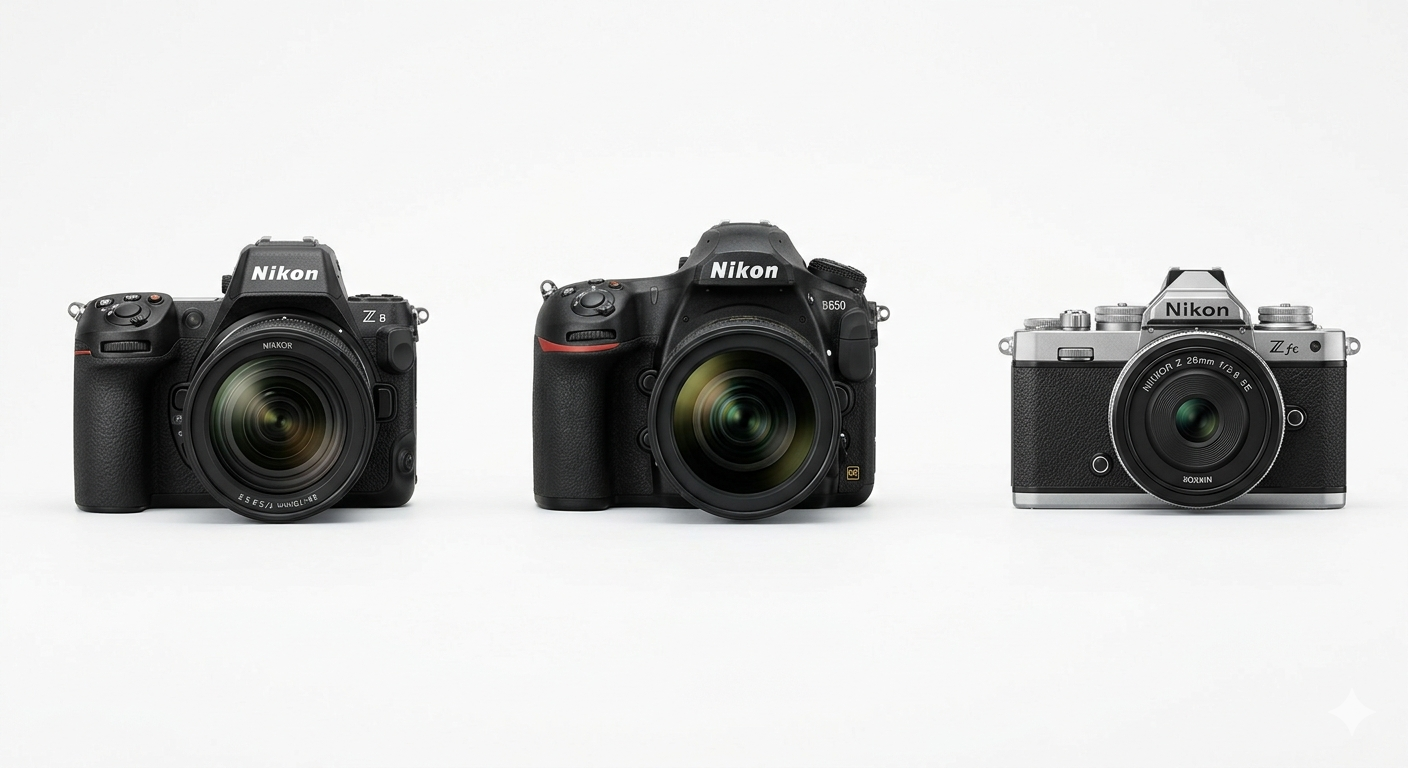
\includegraphics[width=0.45\textwidth]{input.png}
    \caption{原始輸入影像 (包含三臺相機與底部陰影)}
    \label{fig:input}
\end{figure}

經過多重門檻值、破洞填補、形態學切斷連結以及區域生長處理後，輸出結果如圖 \ref{fig:output} 所示。

\begin{figure}[H]
    \centering
    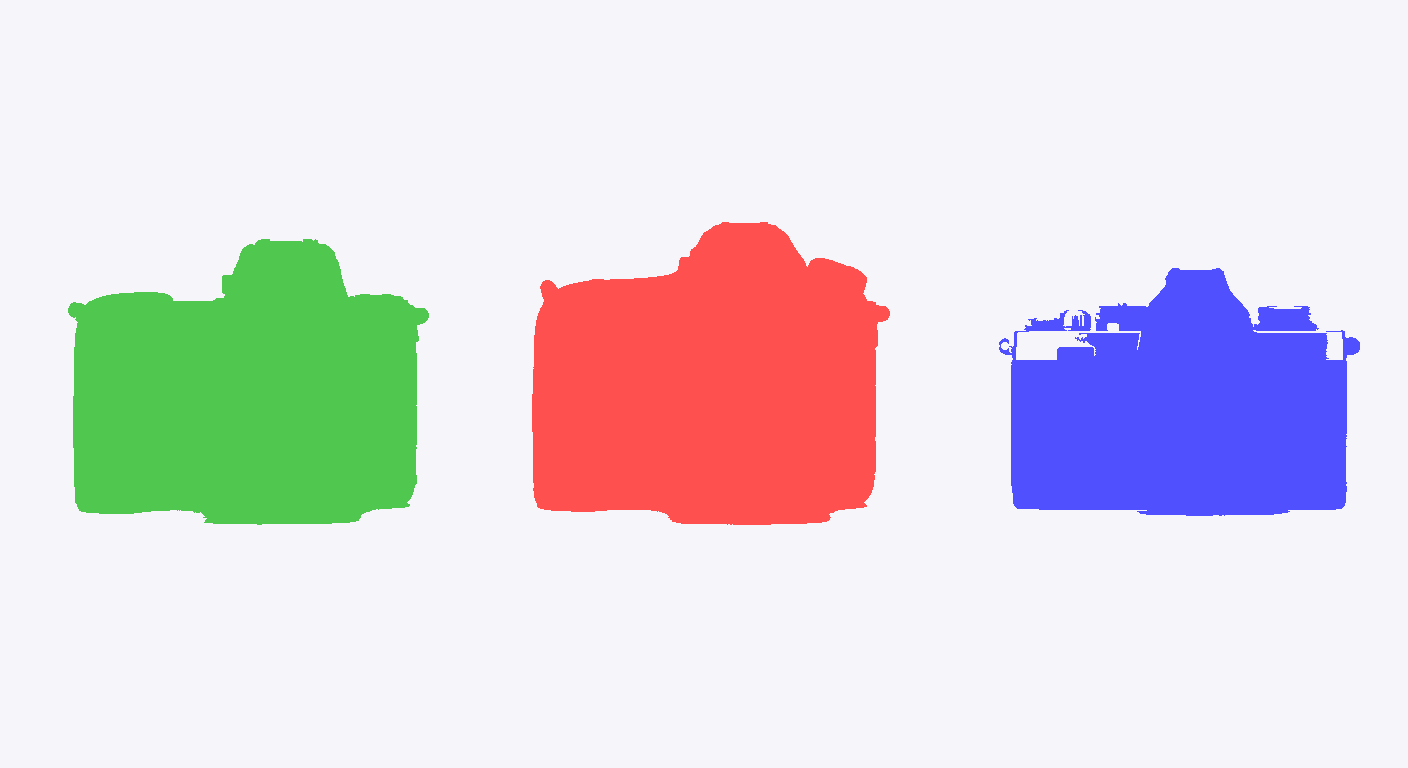
\includegraphics[width=0.45\textwidth]{output.png}
    \caption{實體分割輸出影像 (成功將三臺相機分離並賦予獨立顏色)}
    \label{fig:output}
\end{figure}

實驗結果顯示，即便 Z fc 具備易與背景混淆的銀色機身，且三臺相機底部存在連綿的陰影，本系統仍能成功將其完美獨立提取，並為每一臺相機分配獨一無二的實體顏色（Instance Color），內部無任何雜點破洞，且背景保持乾淨統一，完全符合實體分割（Instance Segmentation）的預期目標。

\section{結論 (Conclusion)}
本作業展示了傳統影像處理技術的極限與突破方法。單純依賴全域亮度特徵的門檻值分割，在面對真實光影與複雜材質時存在先天缺陷。然而，透過巧妙地結合空間資訊（形態學運算）與拓撲特徵（連通元件標記與區域生長），我們能夠大幅提升傳統演算法的強健性（Robustness），達成接近深度學習模型的完美分割效果。

\end{document}